
\section{Lipids}

The solubility of lipids at room temperature are tested. For this experiment the cover glasses are coated with lipids. Then a first before picture was taken. Then the cover glass is given into a small container with the potential solvent. Within 15 minutes, the cover glass is removed and compared under the microscope with the picture taken before. If streaks created from lipids are still as visible as before, the lipids are categorized as insoluble in this solution. If the streaks partially dissapeared and/or are less visible, the lipids are categorized as partially soluble in this solution. Last if the streaks completely disappear, the lipids are assinged as soluble in the solution (Table \ref{table:LoeslichkeitRaumtemperatur}).


\begin{table}[h]
	\centering
	\begin{tabular}{|l|c|c|}
		\hline
		potential solvent & solubility EGG-PC & solubility DOPC \\
		\hline
		\hline
		4-Methyl Pentene & complete & N/A  \\ 
		\hline
		3-Methyl Pentene & partially & no \\
		\hline
		1-Pentene & no & no \\
		\hline
		Isopentane & no & partially\\
		\hline
		1-Propanol & complete & complete\\
		\hline
		Pentane & complete & no\\
		\hline
		Ethanol & N/A & complete\\
		\hline
	\end{tabular}
	\caption{list of tested potential solvent and result of solubility tests at room temperature. complete indicates solvents, which are able to visibly solve all lipids off a cover glass, partially indicates solutions which are able to solve lipids only partially, no stands for solutions which show no visible solubility of tested lipid.}
	\label{table:LoeslichkeitRaumtemperatur}
\end{table}

This experiment shows that 3 solvent exist for EGG-PC as well as DOPC (Table \ref{table:LoeslichkeitRaumtemperatur}). Following those results, these solvents are tested regarding solubility at temperatures of -140°C. As not all solutions are liquid at -140°C (Table \ref{table:SchmelztemperaturLösungsmittel}), they are tested at higher temperatures in which they are still liquid. Also they are tested as mixtures with other solvents with a lower melting point, in hope the resulting solution has a lower melting point between both mixed solvents. Additionally all lipids are tested in liquid ethane.

This experiment shows that no tested solvent was able to solve lipids at -140°C and a short time frame (Table \ref{table:Cryoloeslichkeit}). Also a redistribution of lipids was visible in all experiments. Because a high solubility at cryogenic temperature is needed for solving lipids in a sacrificial layer, none of these tested solvents can be picked as solvents to solve a sacrificial layer. (begründung vielleicht???) as the process of solving lipids are generally exothermic, other ways of removing ice were tested.

\begin{table}[h]
	\centering
	\begin{tabular}{|c|c|}
		\hline
		solvent & melting point in °C \\
		\hline
		\hline
		4-Methyl Pentene & -154 \\ 
		\hline
		3-Methyl Pentene & -154 \\
		\hline
		1-Pentene & -165 \\
		\hline
		Isopentane & -160 \\
		\hline
		1-Propanol & -126 \\
		\hline
		Pentane & -129 \\
		\hline
		Ethanol & -114 \\
		\hline
	\end{tabular}
	\caption{Melting Point in °C for tested solvents.}
	\label{table:SchmelztemperaturLösungsmittel}
\end{table}

\begin{table}[h]
	\begin{subtable}{\linewidth}
		\centering
		\begin{tabular}{|c|c|}
		\hline
		Solvent & Result \\
		\hline
		Pentane & Lipids solved 3h at -125°C \\
		\hline
		4-methyl pentene & insoluble \\
		\hline
		\makecell{1:1 volume ratio\\ HFE to 1-Propanol} & \makecell{did not mix,\\ 1-Propanol froze,\\ insufficient solubility}\\
		\hline
		Flüssiges Ethan & insoluble\\
		\hline
		\end{tabular}
		\caption{EGG-PC}
		\label{table:EGG-PCCryoloeslichkeit}
	\end{subtable}
	\begin{subtable}{\linewidth}
		\centering
		\begin{tabular}{|c|c|}
		\hline
		Solvent & Result \\
		\hline
		\makecell{1:4 volume ratio\\ 1:2 molar ratio\\ Ethanol to Isopentane} & insufficient solubility\\
		\hline
		\makecell{1:2 volume ratio\\ 1:1 molar ratio\ 1-Propanol to Isopentane} & insoluble \\
		\hline
		Isopentane & insufficient solubility\\
		\hline
		1-Propanol & \makecell{at -130°C\\ insufficient solubility}\\
		\hline
		Flüssiges Ethan & insoluble \\
		\hline
		\end{tabular}
		\caption{DOPC}
		\label{table:DOPCCryoloeslichkeit}
	\end{subtable}
	\label{table:Cryoloeslichkeit}
\end{table}

\section{Finger}
For this section, cover glass coated in Parylene are used. The cover glass is then dipped in solution containing lipids for a lipid coating. A ice layer with fluoriscine is frozen with either plunge-freezing or using a pincer and liquid nitrogen. Additionally, the "finger" is used as tool to try lifting off a piece of ice from the frozen layer on top of the lipids.

\subsection{Finding right dosage of HFE}
A Pipette was used to dose HFE for finding the correct amount of HFE to use 

	
\subsection{Temperature over applied force}

HFE GETS HARDER OVER TEMPERATURE

\subsection{Tensile mode vs Shear mode}

In experiments it was observed that pulling sideways will always result in breaking HFE off the finger.

\subsection{Detaching ice with finger of plunge freezed samples}

Next observed possible factor is the thickness of the ice layer. In the following, samples freezed with a plunge-freezer are compared to samples freezed with a pincer in liquid nitrogen. The results are categorized in 4 categories: Not successful pulls don't have visible changes of the flourescent ice layer, Partially successes are visible breaks or clear movement of ice parts on the ice layer, Successful liftoff is a missing piece and a visible piece on the finger, which could be used for future steps. In the results, there is no difference between Hand freezed and plunge-freezed samples regarding detachability. Therefore Ice thickness is not a factor which makes detaching ice easier. As both methods don't show success in detaching ice pieces, it could still be a relevant factor but not a thing which should make a certain solution magically work xD

\begin{table}
	\centering
	\begin{tabular}{|c|c|c|}
		\hline
		Category & Hand-freezed & Plunge-freezed \\
		\hline
		\hline
		count executed tries & 4 & 4\\
		\hline
		unsuccessful & 3 & 3\\
		\hline
		breaks/movement of ice & 1 & 1\\
		\hline
		piece lifted with finger & 0 & 0\\
		\hline		
	\end{tabular}
	\caption{Comparison of detachability between hand-freezed and plunge-freezed samples}
\end{table}

\section{PDMS}

Now two mixture ratios of PDMS are compared. For this, samples where coated with 4:1 and 1:2 curing agent to base coat weight ratio. Also for ..., glass without pdms is used. The pulling mashine was used to determine the max force. A plexiglass stamp was used for pulling off the PDMS layer. UV Glue was used to fixate the plexiglass onto the PDMS and is cured with 3 min UV exposure. After pulling, the Area of the separating layers is determined via microscope. Then the max pulling tension is calculated. This was repeated several times. The Result shows, that glass is hardest do pull off. Then 4:1 is harder to separate than 1:2 (Fig. \ref{fig:vgl4:1zu1:2zuGlas}). In literature, 1:2 weight ratio should have a lower adhesion force on ice too\cite{IbanezIbanez.2022}. For those reasons, 1:2 was picked to continue experiments with plasma treatment.

\begin{figure}
	\centering
	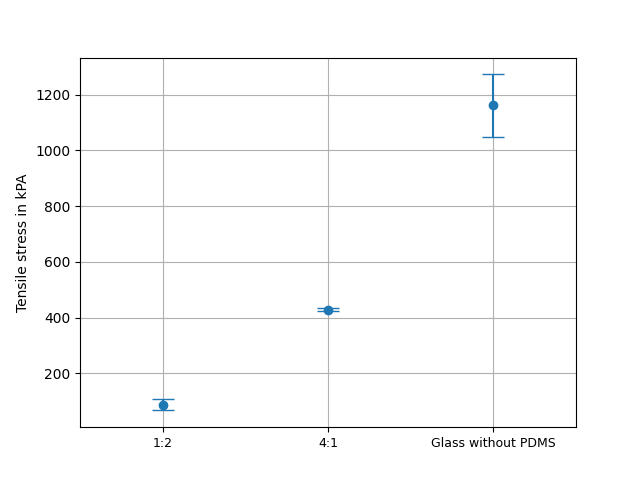
\includegraphics[width=14cm]{plotVGLZugspannungPDMSMischungsverhaeltnisse}
	\caption{Comparison 4:1, 1:2 Base coat to curing Agent and glass without PDMS}
	\label{fig:vgl4:1zu1:2zuGlas}
\end{figure}

\begin{figure}
	\centering
	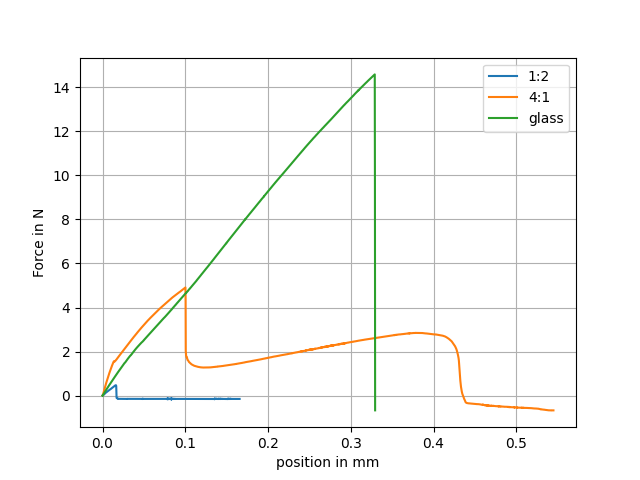
\includegraphics[width=14cm]{ForceOverTime}
	\caption{force over Time}
\end{figure}

In the next experiment, the effect of plasma curing is investigated. The same setup is used. Samples with a 2:1 weight ratio are additionally plasma treated before quickly clamping on the pulling mashine. Even with low repetition rates, a clear tendency can be observed. With lower and stronger plasma treatment, the durable the PDMS Layer gets (Fig. \ref{fig:PlotPlasmaAktivierung}). Over the whole range, The needed stress sextubles. Because the repititon rate is low, the exact values should be treated cautiosly. Also the results are not applicable to other mixture ratios, as different behaviour in plasma activation was observed between 2:1 and 4:1 weight ratio. also no glass-like state was observed in 2:1 weight ratio mixture.


\begin{figure}[h]
	\centering
	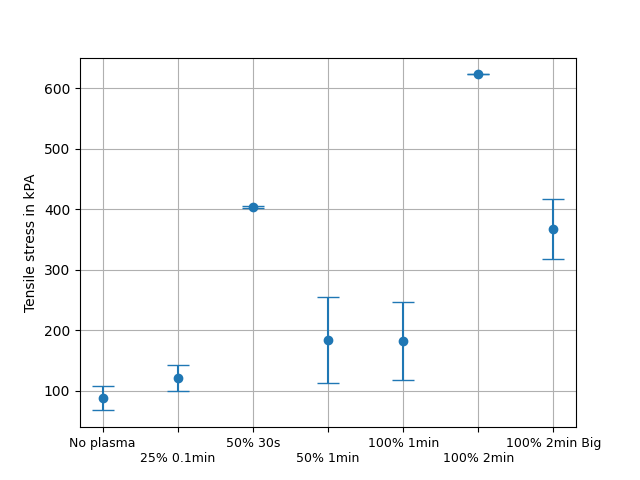
\includegraphics[width=14cm]{plot2_1PlasmaAktivierung}
	\caption{PDMS 2:1 Comparison between various Plasma curing strengths and durations.}
	\label{fig:PlotPlasmaAktivierung}
\end{figure}



